\documentclass[]{beamer}
%\documentclass{article}
%\usepackage{beamerarticle}

\mode<presentation>
{
  \usetheme{Warsaw}
  % or ...

  \setbeamercovered{transparent}
  % or whatever (possibly just delete it)
}


\usepackage[english]{babel}
% or whatever

\usepackage[utf8]{inputenc}
% or whatever

\usepackage{times}
\usepackage[T1]{fontenc}

%%%%%%%%%%%%%%%%%%%%%%%%%%%%%%%%%%
%%                         PACKAGES                      %%
%%%%%%%%%%%%%%%%%%%%%%%%%%%%%%%%%%
\usepackage{hyperref,ctable}
\usepackage{graphicx}
\usepackage{tikz}                    % For flowchart
\usetikzlibrary{shapes,arrows} % For flowchart


%%%%%%%%%%%%%%%%%%%%%%%%%%%%%%%%%%
%%                           COLORS                        %%
%%%%%%%%%%%%%%%%%%%%%%%%%%%%%%%%%%
%AU COLORS
\definecolor{aublue}{RGB}{25,33,129}
\definecolor{aured}{RGB}{244,28,31}

%Red
%\setbeamercolor{titlelike}{bg=aured,fg=white}
\setbeamercolor{structure}{bg=black!25!aured, fg=aured}
%\setbeamercolor*{palette primary}{fg=white,bg=aured}
%\setbeamercolor*{palette quaternary}{fg=white,bg=aublue}

%Blue
\setbeamercolor{titlelike}{bg=aublue,fg=white}
%\setbeamercolor{structure}{bg=black!25!aublue, fg=aublue}
\setbeamercolor*{palette primary}{fg=white,bg=aublue}
\setbeamercolor*{palette quaternary}{fg=white,bg=black!75!aublue}

\setbeamercolor{local structure}{fg=aured,bg=gray!60!aured}
\setbeamercolor{alerted text}{fg=aured}

\newenvironment{concept}[1]%
	{
	\setbeamercolor{background canvas}{bg=aured!10!white}%
	\setbeamercolor{frametitle}{bg=aured}%
	\setbeamercolor{frametitle right}{bg=aured}
	\setbeamercolor{alerted text}{fg=aured}%
	\begin{frame}{Concept}%
	\alert{\bfseries \large #1\\[2em]}}{%
	\end{frame}%
	}


%%%%%%%%%%%%%%%%%%%%%%%%%%%%%%%%%%
%%                         GRAPHICS                       %%
%%%%%%%%%%%%%%%%%%%%%%%%%%%%%%%%%%
%\graphicspath{{/Users/bader/work/Presentations/Images/}}}}


%%%%%%%%%%%%%%%%%%%%%%%%%%%%%%%%%%
%%                        COMMANDS                       %%
%%%%%%%%%%%%%%%%%%%%%%%%%%%%%%%%%%
\newcommand{\strong}[1]{\textbf{#1}}
\AtBeginSection[]{
  \begin{frame}
  \vfill
  \centering
  \begin{beamercolorbox}[sep=8pt,center,shadow=true,rounded=true]{title}
    \usebeamerfont{title}\insertsectionhead\par%
  \end{beamercolorbox}
  \vfill
  \end{frame}
}



%%%%%%%%%%%%%%%%%%%%%%%%%%%%%%%%%%
%%                     PRESENTATION                   %%
%%%%%%%%%%%%%%%%%%%%%%%%%%%%%%%%%%
\title{Introduction to R}

\author[Bader--SOCY 625]
{Michael D.~M.~Bader}

\institute 
{
  Practicum in Sociological Research (SOCY 625)
}
% - Use the \inst command only if there are several affiliations.
% - Keep it simple, no one is interested in your street address.

\date % (optional)
{Week 1}

\subject{Practicum in Sociological Research Slides}
% This is only inserted into the PDF information catalog. Can be left
% out.

% If you have a file called "university-logo-filename.xxx", where xxx
% is a graphic format that can be processed by latex or pdflatex,
% resp., then you can add a logo as follows:

%\logo{\includegraphics[height=1cm]{../../Images/au_logo_50by51px}}
%\logo{\includegraphics[height=1cm]{../../Images/au_logoname_300}}
\logo{\includegraphics[height=1cm]{/Users/bader/work/Presentations/Images/au_logoname_300}}

\subject{Intro to Survey Methods}
% This is only inserted into the PDF information catalog. Can be left
% out. 



% If you have a file called "university-logo-filename.xxx", where xxx
% is a graphic format that can be processed by latex or pdflatex,
% resp., then you can add a logo as follows:

% \pgfdeclareimage[height=0.5cm]{university-logo}{university-logo-filename}
% \logo{\pgfuseimage{university-logo}}



% Delete this, if you do not want the table of contents to pop up at
% the beginning of each subsection:
%\AtBeginSubsection[]
%{
%  \begin{frame}<beamer>{Outline}
%    \tableofcontents[currentsection,currentsubsection]
%  \end{frame}
%}


% If you wish to uncover everything in a step-wise fashion, uncomment
% the following command: 

%\beamerdefaultoverlayspecification{<+->}
\begin{document}
\maketitle
\begin{frame}
R is both: 
\begin{minipage}{.6\textwidth}
\begin{itemize}
\item Statistical computing software
\item Full-fledged programming language
\end{itemize}
\end{minipage}\begin{minipage}{.39\textwidth}

\includegraphics[width=\textwidth]{images/Rlogo.png}
\end{minipage}
\end{frame}

\begin{frame}
So why make you learn something that's harder than what you have already learned? 
\begin{itemize}
\item R is open source, which means that many different people can help extend the language to do common tasks or specialized analysis\pause
\item R has a large user base, so there are lots of places to receive help online, e.g. \url{http://rseek.org/} and \href{https://stackoverflow.com/questions/tagged/r}{Stack Overflow}.\pause
\item R is the future of statistical software; employers will be increasingly moving to R 
\end{itemize}
\end{frame}

\begin{frame}
So why make you learn something that's harder than what you have already learned?
\begin{center}
\begin{tabular}{lrl} \toprule
SAS\footnote{\tiny For SAS Analytics Pro \url{https://www.sas.com/en_us/software/analytics-pro.html}; January 20, 2018} & \$9,720.00 & + Windows only \\
SPSS\footnote{\tiny \url{https://www.ibm.com/products/spss-statistics/pricing}; January 20, 2018} & \$99.00\slash month & + \$237.00/month add-ons \\
Stata\footnote{\tiny Stata 15 government \& nonprofit pricing \url{https://www.stata.com/order/new/gov/single-user-licenses/dl/}; January 20, 2018} & \$1,695.00 & + \$300 for large datasets \\
R & \$0.00 & \\ \bottomrule
\end{tabular}
\end{center}

\end{frame}

\begin{frame}
\includegraphics[width=.5\linewidth]{images/RLogo.png}\\[3em]

{\LARGE \url{https://www.r-project.org/}}
\end{frame}


\begin{frame}
\includegraphics[width=.5\linewidth]{images/RStudioLogo.png}\\[3em]

{\LARGE \url{https://www.rstudio.com/}}
\end{frame}

\begin{frame}[plain]
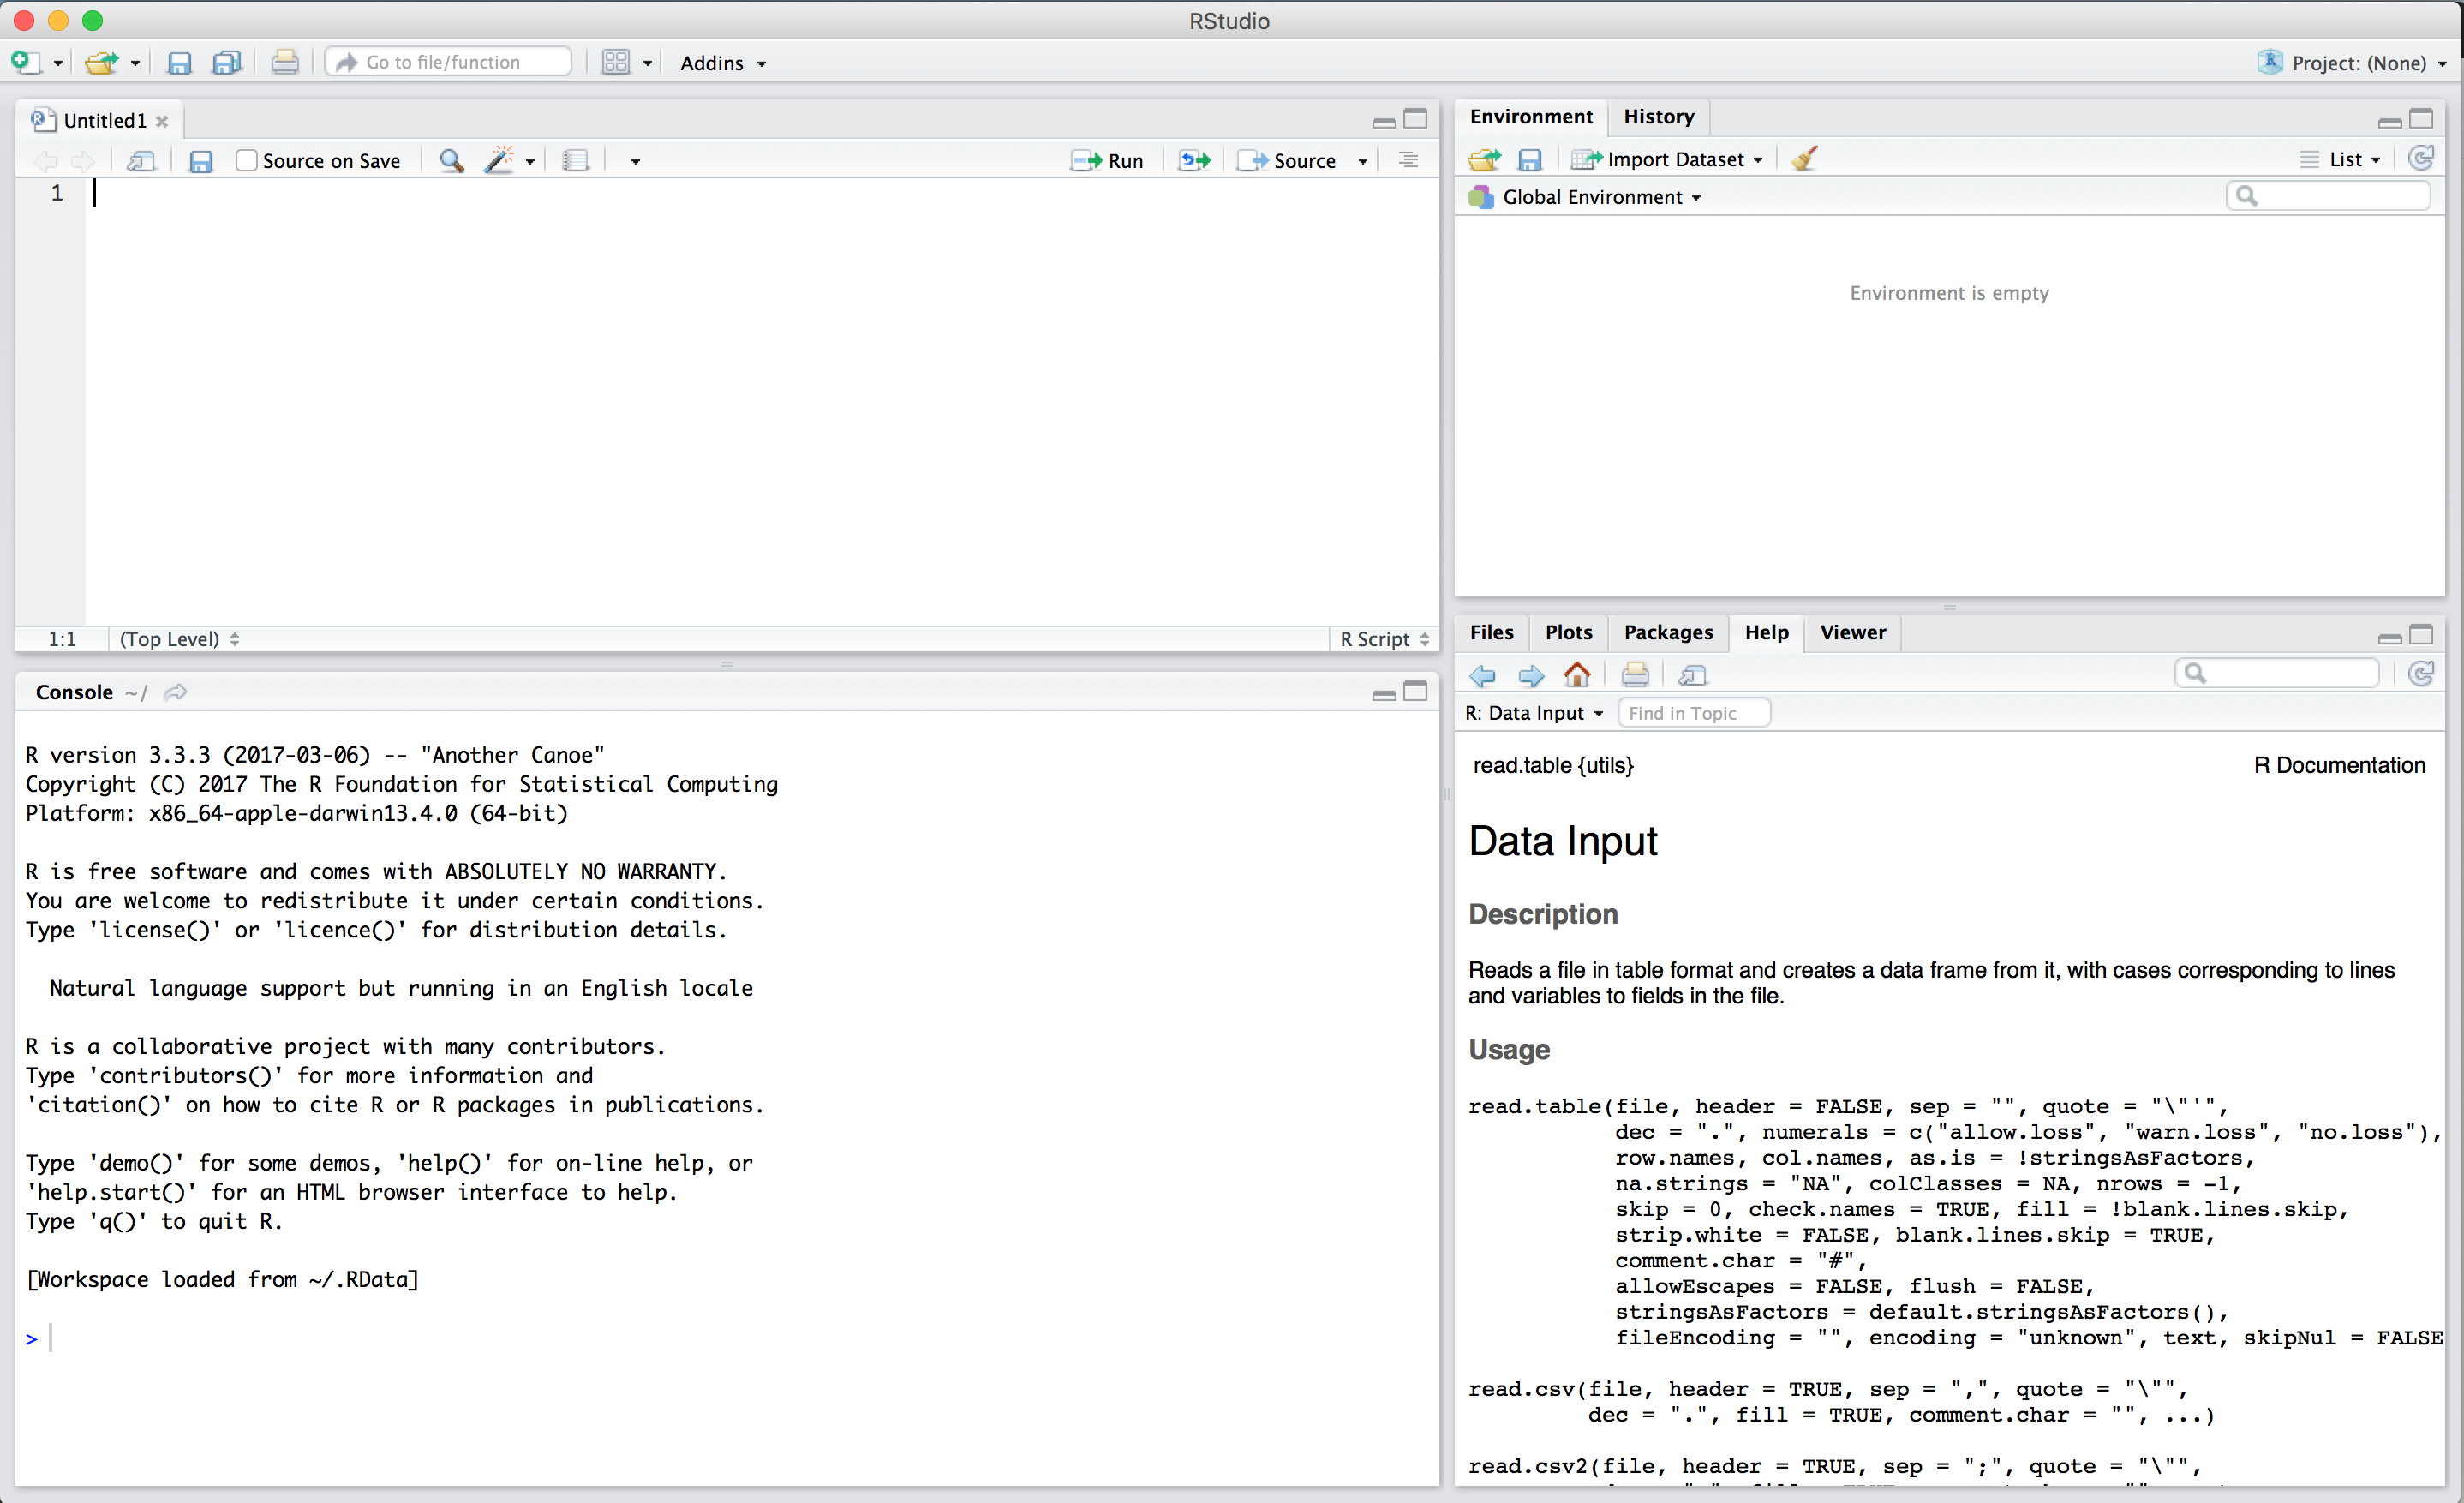
\includegraphics[width=\linewidth]{images/RStudioWorkspace.png}
\begin{tikzpicture}[overlay]
      \node[draw=red,fill=white,name=tar,text=red,outer sep=6pt] at 
                                                        (-.67\linewidth,5) {Source (ctrl-1)};
      \node[draw=red,fill=white,name=tar,text=red,outer sep=6pt] at 
                                                        (-.67\linewidth,2) {Console (ctrl-2)};
      \node[draw=red,fill=white,name=tar,text=red,outer sep=6pt] at 
                                                        (-.25\linewidth,5) {Environment};
	\node[draw=red,fill=white,name=tar,text=red,outer sep=6pt] at 
                                                        (-.25\linewidth,2) {View};

                                                        
\end{tikzpicture}
\end{frame}

\begin{frame}
\textbf{\alert{Do not use spaces in directory or file names:}}\\[2em]

{\small \texttt{/Users/bader/My Documents/Homework/Homework 1.R}}\\[2em]

Is worse than \\[2em]

{\small \texttt{/Users/bader/work/Homework/Homework1.R}}

\end{frame}


\end{document}


